\documentclass[a4paper,12pt]{article}
\usepackage[ngerman]{babel}
\usepackage{multirow}
\usepackage{xltxtra}
\usepackage[utf8x]{inputenc}
\usepackage{fontspec}
\usepackage{eurosym}
\usepackage{graphicx}
\usepackage[paper=a4paper,left=25mm,right=25mm,top=25mm,bottom=25mm]{geometry}
\usepackage{makecell}
\usepackage[table]{xcolor}
\usepackage{float}
\usepackage[normalem]{ulem}
\usepackage{xcolor,colortbl}
\definecolor{Gray}{gray}{0.85}
\usepackage[automark]{scrlayer-scrpage}
\usepackage[
	colorlinks=true,
	urlcolor=blue,
	linkcolor=green
]{hyperref}
\setlength{\parindent}{0em}
\setlength{\parskip}{1ex}
\pagestyle{scrheadings}
\clearscrheadfoot
\usepackage[defaultsans]{droidsans}
\renewcommand*\familydefault{\sfdefault}
\begin{document}
\input{theme.tex}
\input{version.tex}
\newcommand{\combineDivisions}{Hinweis: Wenn weniger als 5 Teams in einer der
Altersgruppen angemeldet sind, hat die Veranstaltungsleitung die Möglichkeit,
Altersgruppen zusammenzulegen. }

\newcommand{\declareExhibition}{Wenn insgesamt weniger als 5 Teams angemeldet
sind kann die Veranstaltung zur Ausstellung erklärt werden. }

\newcommand{\robotRequirements}{Autonomer Roboter, basierend auf einer
beliebigen Plattform, der \euro{1.500} oder weniger kostet und die folgenden
Designbedingungen erfüllt, die beim Check-In überprüft werden:}


\newcommand{\tournamentScoring}{
\begin{figure}[H]
	\centering
	\def\svgwidth{\columnwidth}
	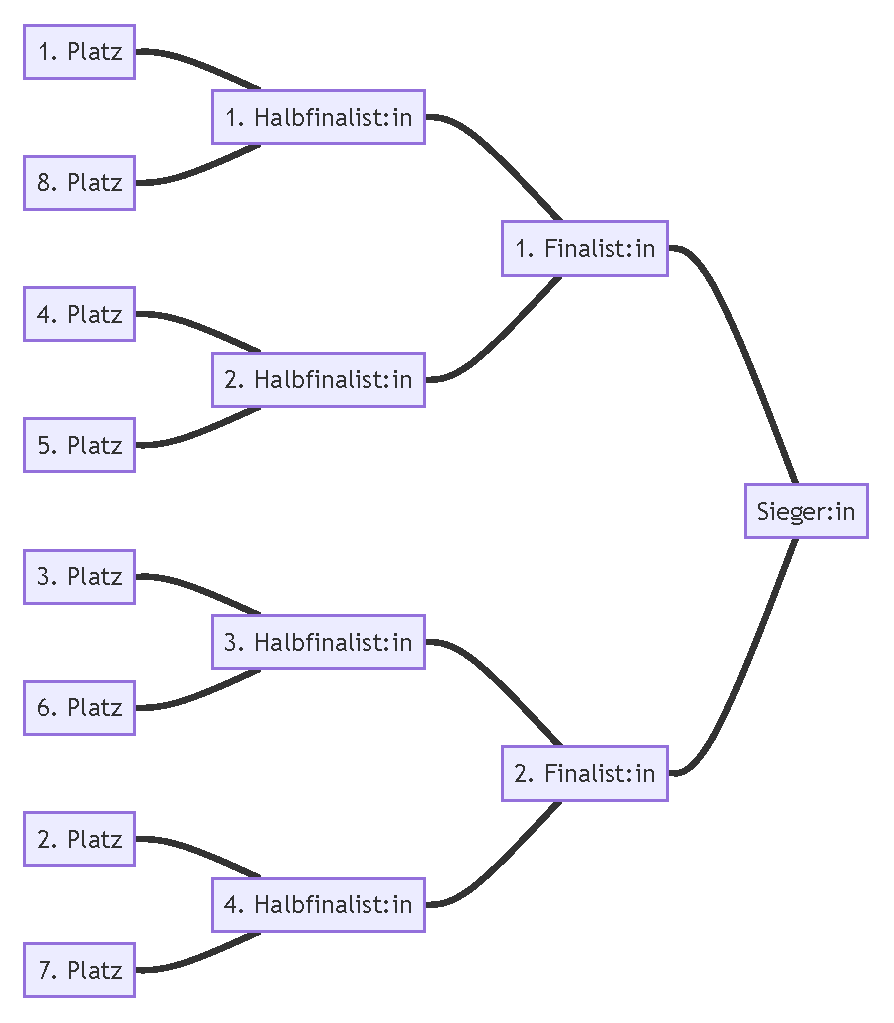
\includegraphics{tournament_score/tournament_score.pdf}
\end{figure}
}

\newcommand{\tournamentQualification}{Die aufsteigenden Teams werden
entsprechend ihrer Gesamtpunktzahl in den Turnierplan eingetragen (unten findet
ihr ein Beispiel für ein typisches Turnier mit 8 Teams). }

\newcommand{\combinedTournament}{
Hinweis: Wenn weniger als 8 Teams in allen Altersgruppen angemeldet sind, hat
die Veranstaltungsleitung die Möglichkeit, den Turnierplan entsprechend
anzupassen.
}

\newcommand{\scoreRuns}{
Die besten (8) Teams, welche am Turnier teilnehmen, werden wie folgt ermittelt:
\begin{itemize}
	\item Die Veranstaltungsleitung legt fest wieviele Läufe pro Team
		offiziell gewertet werden dürfen.
	\item Davon gehen die besten Wertungen in die Gesamtpunktzahl ein.
	\item Die Veranstaltungsleitung legt fest wieviele der offiziell
		gewerteten Läufen in die Gesamtpunktzahl eingehen.
	\item Auf Grundlage dieser Gesamtpunktzahl werden die besten Teams
		ermittelt, welche am Turnier teilnehmen.
\end{itemize}
}

\newcommand{\lightConditions}{
Die Challenge kann in Bereichen mit natürlichen Licht stattfinden, welches die
Lichtverhältnisse auf dem Spielplan verändern kann. Teams sollten darauf
vorbereitet sein, diese natürlichen Bedingungen zu meistern. }

\ohead{Regelstand: \commitDate, id: \commitID}
\title{\tagYear\ Jousting Challenge Regeln}

\makeatletter
\let\inserttitle\@title
\makeatother
\begin{center}
	\rrgerLogo
	\huge                      % Schriftgröße einstellen
	\bfseries                   % Fettdruck einschalten
	\\
	\inserttitle
\end{center}

\section{Ziel}
Entwerfe, baue und programmiere einen Linienfolger, der einen Ritter mitführen
kann (leicht gehalten von einem Magneten auf einer Metallplatte), welcher in
einem Lanzenstechen (sog. Tjost) den gegnerischen Ritter nur mithilfe einer
Lanze zu Boden werfen kann.

\section{Wer kann teilnehmen?}
Teams aus 2 bis 4 Spieler:innen in \textbf{getrennten Altersgruppen}:
\begin{itemize}
	\item Grundschule (ES)
	\item Mittelstufe (MS)
\end{itemize}
\combineDivisions

\section{Anforderungen}
\robotRequirements
\begin{itemize}
	\item Der Roboter kann demonstieren, dass er ein Linienfolgerprogramm
		ausführt indem er der Jousting-Bahn vom Start entlang der
		Kurve bis zur 100 Punkte Linie folgt.
	\item Die Ritterbefestigungsstruktur (Marmeladenglassdeckel) kann mit
		jedem beliebigen Material befestigt werden. Die Art der
		Befestigung darf dem Ritter keine zusätzliche Stütze bieten und
		keine zusätzliche magnetische Haftkraft erzeugen, die dem
		Ritter hilft, an der Struktur befestigt zu bleiben.
	\item Die Ritterbefestigungsstruktur darf sich maximal 10 cm vor dem
		Roboter befinden und maximal eine Höhe von 10 cm über dem Boden
		habe
	\item Der Körper des Ritters ist auf dem erforderlichen Metalldeckel
		völlig freistehend, daher sind KEINE umgebenden Stützsysteme um
		den Metalldeckel herum erlaubt.
	\item Der Ritter ist mit einem rundem Knopfmagneten mit einer Haftkraft
		von 800g an der Metallplatte befestigt.
	\item Es muss ein Linienfolgerprogramm mit einem oder mehreren Sensoren
		verwendet werden welches den Roboter führt
	\item Während der Vorbereitung sind jegliche offizielle Ritter erlaubt.
		Während der Qualifikation oder des Turniers muss jedoch der
		offizielle 2023 Jousting Knight verwendet werden (wird an der
		Bahn für beide Teams bereitgestellt).
	\item Das Volumen des Roboter darf 65030 cm$^{3}$ \textbf{nicht}
		überschreiten.
\end{itemize}
\section{Allgemeine Spielregeln}
\begin{enumerate}
	\item Grundschul- und Mittelschulteams spielen in getrennten
		Altersgruppen.
	\item Ein Linienfolgerprogramm muss die Bewegung des
		Roboters steuern.
	\item Währed der Wertungsphase gibt es keine festgelegten Gegner:innen,
		geht einfach zu irgendeinem Spielfeld um Gegner:innen zu
		finden
	\item Führt während der Wertungsphase so viele Tjosts durch, wie ihr
		bereit seid (Grundschul- und Mittelschul-Tjostteams benötigen 5
		gemeldete Wertungen).
	\item \textbf{Nur die Lanze} darf den Ritter herunterstoßen. Sollte der
		Ritter durch etwas anderes heruntergestoßen werfen, so wird mit
		der nächsten Tjost fortgefahren (außer es handelt sich um die
		5. Tjost).
	\item Während eines Tjostkampfes sind bis zu 5 Versuche erlaubt, den
		gegnerischen Ritter herunterzustoßen.
	\item  Wenn nach fünf (5) Versuchen kein Ritter herunter gestoßen
		wurden, gilt der Tjost als unentschieden. Beide Teams
		überlassen das Spielfeld den wartenden Teams.
	\item Wenn beide Ritter zu Boden fallen, gilt der Ritter, welcher lt.
		Punktrichter:innen zuletzt den Boden berührt als Gewinner.
	\item \textbf{Nur} die Lanze darf die Mittellinie des Spielfeldes
		überqueren (\textasciitilde13 cm von den jeweiligen 2
		parallelen Linien entfernt).
\end{enumerate}

\section{Challenge Spezifikation}
\begin{enumerate}
	\item Zwei parallele ungefähr 2,5 cm breite Linien auf weißer PVC-Plane.
	\item Jede Linie hat zu Beginn eine leichte Kurve.
	\item Ein Meterstab \emph{kann durch die Schiedsrichter} unter der
		Plane entlang der Mittellinie als Schranke (sog. "Tilt")
		platziert werden.
	\item Es gibt drei Wertungszonen:
		\begin{itemize}
			\item $150$ Punkte ($0,0 cm$ bis $\approx15 cm$ vom Start)
			\item $100$ Punkte ($\approx15 cm$ bis $\approx30 cm$ vom Start)
			\item $50$ Punkte ($\approx30 cm$ bis $\approx91 cm$ vom Start).
		\end{itemize}
\end{enumerate}
\includegraphics[width=1\textwidth]{images/track.png}

\section{Punktevergabe}
\begin{enumerate}
	\item Den Teams wird dringend empfohlen, in der ersten Hälfte der
		Wertungsphase mit der Bewertung ihrer Roboter zu beginnen, um
		sicherzustellen, dass sie bis zur zweiten Hälfte der
		Wertungsphase die Mindestanzahl von 5 Läufen erreicht haben.
\end{enumerate}

\section{Turnier-Wertung}
\begin{enumerate}
	\item Die volle Punktzahl wird \textbf{nur} vergeben, wenn ihr den
		gegnerischen Ritter im \textbf{ersten} von fünf Veruschen
		herunterstoßt. Jeder folgende Versuch verringert die Punkte.
		\textbf{Siehe Tabelle unten}.
	\item Höhere Punktezahlen werden erzielt, je näher das Herunterwerfen
		an der Startposition gelingt.
	\item Wenn der Ritter (\emph{nicht die Lanze}) zwischen 2
		Punktebereichen liegt, zählt die höhere Punktezahl.
\end{enumerate}

\pagebreak
\section{Punktetabelle}
\begin{center}
\begin{tabular}{|c|c|c|c|c|c|c|c|} \hline
	\multicolumn{8}{|l|}{NUR WENN ein Ritter mit der Lanze des gegnerischen Ritters heruntergestoßen wurde}\\
	\multicolumn{8}{|l|}{bekommt der Sieger Punkte}\\
	\multicolumn{8}{|l|}{}\\
	\multicolumn{8}{|l|}{Definition: Tojst - der Versuch beider Roboter den gegnerischen Ritter herunterzustoßen}\\
	\multicolumn{8}{|l|}{}\\
	\multicolumn{8}{|l|}{Jedes Team hat 5 Tjosts um den gegnerischen Ritter herunterzustossen} \\ \hline
	\multicolumn{2}{|c|}{\multirow{2}{*}{\textbf{Punkte pro Tjost}}} & \textbf{1. Tjost} & \textbf{2. Tjost} & \textbf{3. Tjost} & \textbf{4. Tjost} & \textbf{5. Tjost} & 5 Tjosts und \\
	\multicolumn{2}{|c|}{}  & (100\%) & (90\%) & (80\%) & (70\%) & (60\%) & kein Sieger? \\
	\cline{1-7}
	\multirow{3}{*}{\textbf{Punkte}} & 150 Zone & 150 & 140 & 130 & 120 & 110 & Unentschieden: \\
	\cline{2-7}
	& 100 Zone & 100 & 90 & 80 & 70 & 60 & Jedes Team \\
	\cline{2-7}
	& 50  Zone& 50 & 40 & 30 & 20 & 10 & 5 Punkte \\
	%\hline
	%\multicolumn{8}{|c|}{Der Verlierer bekommt 0 Punkte}\\
	\hline
\end{tabular}
\end{center}

\pagebreak
\section{Tunierplan}
\begin{itemize}
	\item Die besten acht Teams jeder Altersgruppe werden an der Endrunde
		teilnehmen.
        \item \tournamentQualification
\end{itemize}
\tournamentScoring
\combinedTournament
\end{document}
